% Options for packages loaded elsewhere
\PassOptionsToPackage{unicode}{hyperref}
\PassOptionsToPackage{hyphens}{url}
\PassOptionsToPackage{dvipsnames,svgnames,x11names}{xcolor}
%
\documentclass[
  letterpaper,
  DIV=11,
  numbers=noendperiod]{scrartcl}

\usepackage{amsmath,amssymb}
\usepackage{iftex}
\ifPDFTeX
  \usepackage[T1]{fontenc}
  \usepackage[utf8]{inputenc}
  \usepackage{textcomp} % provide euro and other symbols
\else % if luatex or xetex
  \usepackage{unicode-math}
  \defaultfontfeatures{Scale=MatchLowercase}
  \defaultfontfeatures[\rmfamily]{Ligatures=TeX,Scale=1}
\fi
\usepackage{lmodern}
\ifPDFTeX\else  
    % xetex/luatex font selection
    \setmainfont[]{Times New Roman}
\fi
% Use upquote if available, for straight quotes in verbatim environments
\IfFileExists{upquote.sty}{\usepackage{upquote}}{}
\IfFileExists{microtype.sty}{% use microtype if available
  \usepackage[]{microtype}
  \UseMicrotypeSet[protrusion]{basicmath} % disable protrusion for tt fonts
}{}
\makeatletter
\@ifundefined{KOMAClassName}{% if non-KOMA class
  \IfFileExists{parskip.sty}{%
    \usepackage{parskip}
  }{% else
    \setlength{\parindent}{0pt}
    \setlength{\parskip}{6pt plus 2pt minus 1pt}}
}{% if KOMA class
  \KOMAoptions{parskip=half}}
\makeatother
\usepackage{xcolor}
\usepackage[top=30mm,left=20mm]{geometry}
\setlength{\emergencystretch}{3em} % prevent overfull lines
\setcounter{secnumdepth}{-\maxdimen} % remove section numbering
% Make \paragraph and \subparagraph free-standing
\makeatletter
\ifx\paragraph\undefined\else
  \let\oldparagraph\paragraph
  \renewcommand{\paragraph}{
    \@ifstar
      \xxxParagraphStar
      \xxxParagraphNoStar
  }
  \newcommand{\xxxParagraphStar}[1]{\oldparagraph*{#1}\mbox{}}
  \newcommand{\xxxParagraphNoStar}[1]{\oldparagraph{#1}\mbox{}}
\fi
\ifx\subparagraph\undefined\else
  \let\oldsubparagraph\subparagraph
  \renewcommand{\subparagraph}{
    \@ifstar
      \xxxSubParagraphStar
      \xxxSubParagraphNoStar
  }
  \newcommand{\xxxSubParagraphStar}[1]{\oldsubparagraph*{#1}\mbox{}}
  \newcommand{\xxxSubParagraphNoStar}[1]{\oldsubparagraph{#1}\mbox{}}
\fi
\makeatother

\usepackage{color}
\usepackage{fancyvrb}
\newcommand{\VerbBar}{|}
\newcommand{\VERB}{\Verb[commandchars=\\\{\}]}
\DefineVerbatimEnvironment{Highlighting}{Verbatim}{commandchars=\\\{\}}
% Add ',fontsize=\small' for more characters per line
\usepackage{framed}
\definecolor{shadecolor}{RGB}{241,243,245}
\newenvironment{Shaded}{\begin{snugshade}}{\end{snugshade}}
\newcommand{\AlertTok}[1]{\textcolor[rgb]{0.68,0.00,0.00}{#1}}
\newcommand{\AnnotationTok}[1]{\textcolor[rgb]{0.37,0.37,0.37}{#1}}
\newcommand{\AttributeTok}[1]{\textcolor[rgb]{0.40,0.45,0.13}{#1}}
\newcommand{\BaseNTok}[1]{\textcolor[rgb]{0.68,0.00,0.00}{#1}}
\newcommand{\BuiltInTok}[1]{\textcolor[rgb]{0.00,0.23,0.31}{#1}}
\newcommand{\CharTok}[1]{\textcolor[rgb]{0.13,0.47,0.30}{#1}}
\newcommand{\CommentTok}[1]{\textcolor[rgb]{0.37,0.37,0.37}{#1}}
\newcommand{\CommentVarTok}[1]{\textcolor[rgb]{0.37,0.37,0.37}{\textit{#1}}}
\newcommand{\ConstantTok}[1]{\textcolor[rgb]{0.56,0.35,0.01}{#1}}
\newcommand{\ControlFlowTok}[1]{\textcolor[rgb]{0.00,0.23,0.31}{\textbf{#1}}}
\newcommand{\DataTypeTok}[1]{\textcolor[rgb]{0.68,0.00,0.00}{#1}}
\newcommand{\DecValTok}[1]{\textcolor[rgb]{0.68,0.00,0.00}{#1}}
\newcommand{\DocumentationTok}[1]{\textcolor[rgb]{0.37,0.37,0.37}{\textit{#1}}}
\newcommand{\ErrorTok}[1]{\textcolor[rgb]{0.68,0.00,0.00}{#1}}
\newcommand{\ExtensionTok}[1]{\textcolor[rgb]{0.00,0.23,0.31}{#1}}
\newcommand{\FloatTok}[1]{\textcolor[rgb]{0.68,0.00,0.00}{#1}}
\newcommand{\FunctionTok}[1]{\textcolor[rgb]{0.28,0.35,0.67}{#1}}
\newcommand{\ImportTok}[1]{\textcolor[rgb]{0.00,0.46,0.62}{#1}}
\newcommand{\InformationTok}[1]{\textcolor[rgb]{0.37,0.37,0.37}{#1}}
\newcommand{\KeywordTok}[1]{\textcolor[rgb]{0.00,0.23,0.31}{\textbf{#1}}}
\newcommand{\NormalTok}[1]{\textcolor[rgb]{0.00,0.23,0.31}{#1}}
\newcommand{\OperatorTok}[1]{\textcolor[rgb]{0.37,0.37,0.37}{#1}}
\newcommand{\OtherTok}[1]{\textcolor[rgb]{0.00,0.23,0.31}{#1}}
\newcommand{\PreprocessorTok}[1]{\textcolor[rgb]{0.68,0.00,0.00}{#1}}
\newcommand{\RegionMarkerTok}[1]{\textcolor[rgb]{0.00,0.23,0.31}{#1}}
\newcommand{\SpecialCharTok}[1]{\textcolor[rgb]{0.37,0.37,0.37}{#1}}
\newcommand{\SpecialStringTok}[1]{\textcolor[rgb]{0.13,0.47,0.30}{#1}}
\newcommand{\StringTok}[1]{\textcolor[rgb]{0.13,0.47,0.30}{#1}}
\newcommand{\VariableTok}[1]{\textcolor[rgb]{0.07,0.07,0.07}{#1}}
\newcommand{\VerbatimStringTok}[1]{\textcolor[rgb]{0.13,0.47,0.30}{#1}}
\newcommand{\WarningTok}[1]{\textcolor[rgb]{0.37,0.37,0.37}{\textit{#1}}}

\providecommand{\tightlist}{%
  \setlength{\itemsep}{0pt}\setlength{\parskip}{0pt}}\usepackage{longtable,booktabs,array}
\usepackage{calc} % for calculating minipage widths
% Correct order of tables after \paragraph or \subparagraph
\usepackage{etoolbox}
\makeatletter
\patchcmd\longtable{\par}{\if@noskipsec\mbox{}\fi\par}{}{}
\makeatother
% Allow footnotes in longtable head/foot
\IfFileExists{footnotehyper.sty}{\usepackage{footnotehyper}}{\usepackage{footnote}}
\makesavenoteenv{longtable}
\usepackage{graphicx}
\makeatletter
\def\maxwidth{\ifdim\Gin@nat@width>\linewidth\linewidth\else\Gin@nat@width\fi}
\def\maxheight{\ifdim\Gin@nat@height>\textheight\textheight\else\Gin@nat@height\fi}
\makeatother
% Scale images if necessary, so that they will not overflow the page
% margins by default, and it is still possible to overwrite the defaults
% using explicit options in \includegraphics[width, height, ...]{}
\setkeys{Gin}{width=\maxwidth,height=\maxheight,keepaspectratio}
% Set default figure placement to htbp
\makeatletter
\def\fps@figure{htbp}
\makeatother

\KOMAoption{captions}{tableheading}
\makeatletter
\@ifpackageloaded{caption}{}{\usepackage{caption}}
\AtBeginDocument{%
\ifdefined\contentsname
  \renewcommand*\contentsname{Table of contents}
\else
  \newcommand\contentsname{Table of contents}
\fi
\ifdefined\listfigurename
  \renewcommand*\listfigurename{List of Figures}
\else
  \newcommand\listfigurename{List of Figures}
\fi
\ifdefined\listtablename
  \renewcommand*\listtablename{List of Tables}
\else
  \newcommand\listtablename{List of Tables}
\fi
\ifdefined\figurename
  \renewcommand*\figurename{Figure}
\else
  \newcommand\figurename{Figure}
\fi
\ifdefined\tablename
  \renewcommand*\tablename{Table}
\else
  \newcommand\tablename{Table}
\fi
}
\@ifpackageloaded{float}{}{\usepackage{float}}
\floatstyle{ruled}
\@ifundefined{c@chapter}{\newfloat{codelisting}{h}{lop}}{\newfloat{codelisting}{h}{lop}[chapter]}
\floatname{codelisting}{Listing}
\newcommand*\listoflistings{\listof{codelisting}{List of Listings}}
\makeatother
\makeatletter
\makeatother
\makeatletter
\@ifpackageloaded{caption}{}{\usepackage{caption}}
\@ifpackageloaded{subcaption}{}{\usepackage{subcaption}}
\makeatother

\ifLuaTeX
  \usepackage{selnolig}  % disable illegal ligatures
\fi
\usepackage{bookmark}

\IfFileExists{xurl.sty}{\usepackage{xurl}}{} % add URL line breaks if available
\urlstyle{same} % disable monospaced font for URLs
\hypersetup{
  pdftitle={Beyond numbers. Multiple Correspondence Analysis},
  pdfauthor={, and },
  colorlinks=true,
  linkcolor={blue},
  filecolor={Maroon},
  citecolor={Blue},
  urlcolor={Blue},
  pdfcreator={LaTeX via pandoc}}


\title{Beyond numbers. Multiple Correspondence Analysis}
\author{Pierre Benz\textsuperscript{1,*} \and Thierry
Rossier\textsuperscript{2,3}}
\date{}

\begin{document}
\maketitle


\textsuperscript{1} École de bibliothéconomie et des sciences de
l'information, Université de Montréal, Montréal, Canada.\\
\textsuperscript{2} Life Course and Inequality Research Centre (LIVES),
University of Lausanne, Lausanne, Switzerland.\\
\textsuperscript{3} Department of Sociology, London School of Economics,
London, United Kingdom.

\textsuperscript{*} Correspondence:
\href{mailto:pierre.benz@umontreal.ca}{Pierre Benz
\textless{}pierre.benz@umontreal.ca\textgreater{}}

\normalsize

\normalsize

\subsection{Description}\label{description}

This document supports the ctrl+R session `Beyond numbers. Multiple
Correspondence Analysis' by Thierry Rossier and Pierre Benz, University
of Lausanne, Lausanne, December 5, 2024.

\subsection{Install packages}\label{install-packages}

\scriptsize

\begin{Shaded}
\begin{Highlighting}[]
\FunctionTok{library}\NormalTok{(soc.ca) }\CommentTok{\# for multiple correspondence analysis}
\FunctionTok{library}\NormalTok{(tidyverse) }\CommentTok{\# for data manipulation}
\FunctionTok{library}\NormalTok{(FactoMineR) }\CommentTok{\# for catdes function (univariate analysis)}
\FunctionTok{library}\NormalTok{(factoextra) }\CommentTok{\# for silhouette analysis (k{-}means clustering)}

\CommentTok{\# to install the packages, please use: }
\CommentTok{\# install.packages(c("soc.ca", "tidyverse", "FactoMineR", "factoextra"))}
\end{Highlighting}
\end{Shaded}

\normalsize

After loading the `soc.ca' package, you can access its basic information
through the help file:

\scriptsize

\begin{Shaded}
\begin{Highlighting}[]
\NormalTok{?soc.ca}
\end{Highlighting}
\end{Shaded}

\normalsize

\subsection{Load data and set `active' and `supplementary'
objects}\label{load-data-and-set-active-and-supplementary-objects}

Use \texttt{?soc.ca} to access basic information about the package in
the `Help' pane. The `Examples' section provides the code needed to load
the `taste' dataset and specify variables as either `active' or `sup'.

\scriptsize

\begin{Shaded}
\begin{Highlighting}[]
\FunctionTok{data}\NormalTok{(taste)}
\FunctionTok{names}\NormalTok{(taste)}
\end{Highlighting}
\end{Shaded}

\begin{verbatim}
[1] "ID"     "Isup"   "TV"     "Film"   "Art"    "Eat"    "Gender" "Age"   
[9] "Income"
\end{verbatim}

\begin{Shaded}
\begin{Highlighting}[]
\CommentTok{\# Create a data frame of factors containing all the active variables (+ remove supplementary individuals)}
\NormalTok{taste          }\OtherTok{\textless{}{-}}\NormalTok{ taste[}\FunctionTok{which}\NormalTok{(taste}\SpecialCharTok{$}\NormalTok{Isup }\SpecialCharTok{==} \StringTok{\textquotesingle{}Active\textquotesingle{}}\NormalTok{), ]}

\FunctionTok{attach}\NormalTok{(taste)}
\NormalTok{active         }\OtherTok{\textless{}{-}} \FunctionTok{data.frame}\NormalTok{(TV, Film, Art, Eat)}
\NormalTok{sup            }\OtherTok{\textless{}{-}} \FunctionTok{data.frame}\NormalTok{(Gender, Age, Income)}
\FunctionTok{detach}\NormalTok{(taste)}
\end{Highlighting}
\end{Shaded}

\normalsize

Alternatively, you can use the tidyverse as follows:

\scriptsize

\begin{Shaded}
\begin{Highlighting}[]
\NormalTok{active }\OtherTok{\textless{}{-}}\NormalTok{ taste }\SpecialCharTok{\%\textgreater{}\%} \FunctionTok{select}\NormalTok{(TV, Film, Art, Eat)}
\NormalTok{sup }\OtherTok{\textless{}{-}}\NormalTok{ taste }\SpecialCharTok{\%\textgreater{}\%} \FunctionTok{select}\NormalTok{(Gender, Age, Income)}
\end{Highlighting}
\end{Shaded}

\normalsize

\textbf{Methodological Note}: Modalities must have a frequency of at
least 5\%. Frequencies below this threshold can distort the factorial
structure, as modalities represented by very few cases tend to diverge
significantly from the broader dataset, leading to disproportionate
influence.

\subsection{Run the MCA}\label{run-the-mca}

Here is the code to run MCA and inspect the results:

\scriptsize

\begin{Shaded}
\begin{Highlighting}[]
\NormalTok{result         }\OtherTok{\textless{}{-}} \FunctionTok{soc.mca}\NormalTok{(active, sup)}
\NormalTok{result}
\end{Highlighting}
\end{Shaded}

\begin{verbatim}
                        Specific Multiple Correspondence Analysis:                         
 
                    Statistics                                   Scree plot               
    Active dimensions:                            12  |  1.     47.6%   ************************
    Dimensions explaining 80% of inertia:          3  |  2.     21.5%   ***********
    Active modalities:                            29  |  3.     11.8%   ******
    Supplementary modalities:                     14  |  4.      7.1%   ****
    Individuals:                                1215  |  5.      5.0%   **
    Share of passive mass:                         0  |  6.      3.0%   **
    Number of passive modalities:                  0  |  7.      1.7%   *

                    The 4 active variables: [No. modalities - share of variance]                    

             TV [8 - 28%]            Film [8 - 28%]             Art [7 - 24%] 
            Eat [6 - 20%]
\end{verbatim}

\normalsize

You need to know the importance of the axes, as well as the list of the
contributive modalities.

\scriptsize

\begin{Shaded}
\begin{Highlighting}[]
\FunctionTok{variance}\NormalTok{(result)}
\end{Highlighting}
\end{Shaded}

\begin{verbatim}

Dim        1.    2.    3.    4.    
Eigen      0.40  0.35  0.32  0.31
Var        6.4   5.6   5.2   4.9
Adj.Var   47.6  21.5  11.8   7.1
Cum %     47.6  69.1  80.9  88.0
\end{verbatim}

\begin{Shaded}
\begin{Highlighting}[]
\FunctionTok{contribution}\NormalTok{(result, }\AttributeTok{dim =} \DecValTok{1}\NormalTok{)}
\end{Highlighting}
\end{Shaded}

\begin{verbatim}

  Dimension 1. (+)  
                        Ctr    Coord
Film: CostumeDrama     12.7     1.33
TV: Tv-News             8.8     0.88
Eat: FrenchRest         8.2     1.27
Film: Documentary       5.4     1.02
TV: Tv-Nature           4.9     0.78

  Dimension 1. (-)  
                        Ctr    Coord
TV: Tv-Soap             8.4    -0.87
Film: Comedy            6.8    -0.75
Art: Portrait           6.3    -1.02
Film: Romance           5.5    -1.03
Eat: IndianRest         5.3    -0.51
Art: ModernArt          5.0    -0.94
TV: Tv-Comedy           4.9    -0.79
Film: Horror            3.8    -1.09
\end{verbatim}

\begin{Shaded}
\begin{Highlighting}[]
\FunctionTok{contribution}\NormalTok{(result, }\AttributeTok{dim =} \DecValTok{2}\NormalTok{)}
\end{Highlighting}
\end{Shaded}

\begin{verbatim}

  Dimension 2. (+)  
                        Ctr    Coord
TV: Tv-Soap            15.1     1.09
Film: Romance           9.1     1.24
Film: Musical           8.4     1.29
Eat: Pub                6.5     0.63
Art: Landscape          5.6     0.39
Eat: Fish&Chips         3.9     0.79
Eat: SteakHouse         3.5     0.78

  Dimension 2. (-)  
                        Ctr    Coord
TV: Tv-Comedy           8.2    -0.96
Art: Impressionism      7.1    -0.99
Art: ModernArt          5.9    -0.96
Eat: IndianRest         4.0    -0.41
Eat: ItalianRest        3.9    -0.54
Film: Horror            3.6    -1.00
\end{verbatim}

\normalsize

You might also be interested in examining the contributions of all
modalities to the axes (e.g., axes 1 and 2).

\scriptsize

\begin{Shaded}
\begin{Highlighting}[]
\FunctionTok{contribution}\NormalTok{(result, }\DecValTok{1}\SpecialCharTok{:}\DecValTok{2}\NormalTok{, }\AttributeTok{mode =} \StringTok{"variable"}\NormalTok{)}
\end{Highlighting}
\end{Shaded}

\begin{verbatim}
The contribution of the active variables
 
 Art                  Dim.1  Dim.2   Freq
 Art: Impressionism     2.0    7.1    125
 Art: Landscape         1.7    5.6    632
 Art: ModernArt         5.0    5.9    110
 Art: PerformanceArt      0      0    105
 Art: Portrait          6.3    2.1    117
 Art: RenaissanceArt    3.0    1.8     55
 Art: StillLife         1.2    0.9     71
 Total                 19.2   23.4   1215
 
 Eat                  Dim.1  Dim.2   Freq
 Eat: Fish&Chips        0.4    3.9    107
 Eat: FrenchRest        8.2    1.4     99
 Eat: IndianRest        5.3    4.0    402
 Eat: ItalianRest       0.0    3.9    228
 Eat: Pub               1.2    6.5    281
 Eat: SteakHouse        0.3    3.5     98
 Total                 15.4   23.2   1215
 
 Film                 Dim.1  Dim.2   Freq
 Film: Action           0.1    0.4    389
 Film: Comedy           6.8    1.3    235
 Film: CostumeDrama    12.7    0.0    140
 Film: Documentary      5.4    0.2    100
 Film: Horror           3.8    3.6     62
 Film: Musical          0.1    8.4     87
 Film: Romance          5.5    9.1    101
 Film: SciFi            0.2    2.7    101
 Total                 34.6   25.7   1215
 
 TV                   Dim.1  Dim.2   Freq
 TV: Tv-Comedy          4.9    8.2    152
 TV: Tv-Drama           1.7    0.0    134
 TV: Tv-Films           2.0    3.3    117
 TV: Tv-Nature          4.9    0.1    159
 TV: Tv-News            8.8    0.0    220
 TV: Tv-Police          0.2    0.8     82
 TV: Tv-Soap            8.4   15.1    215
 TV: Tv-Sport           0.0    0.1    136
 Total                 30.9   27.6   1215
Average contribution per modality: 3.4
Total number of individuals: 1215
\end{verbatim}

\normalsize

\subsection{Plot the results}\label{plot-the-results}

You can get all the necessary information about the plotting functions
by using ?map.active, ?map.ctr, ?map.sup, ?map.ind.

\subsubsection{Cloud of active
modalities}\label{cloud-of-active-modalities}

\scriptsize

\begin{Shaded}
\begin{Highlighting}[]
\FunctionTok{map.active}\NormalTok{(}
\NormalTok{  result,}
  \AttributeTok{dim =} \FunctionTok{c}\NormalTok{(}\DecValTok{1}\NormalTok{, }\DecValTok{2}\NormalTok{),}
  \AttributeTok{point.shape =} \StringTok{"variable"}\NormalTok{,}
  \AttributeTok{point.alpha =} \FloatTok{0.8}\NormalTok{,}
  \AttributeTok{point.fill =} \StringTok{"whitesmoke"}\NormalTok{,}
  \AttributeTok{point.color =} \StringTok{"black"}\NormalTok{,}
  \AttributeTok{point.size =} \StringTok{"freq"}\NormalTok{,}
  \AttributeTok{label =} \ConstantTok{TRUE}\NormalTok{,}
  \AttributeTok{label.repel =} \ConstantTok{FALSE}\NormalTok{,}
  \AttributeTok{label.alpha =} \FloatTok{0.8}\NormalTok{,}
  \AttributeTok{label.color =} \StringTok{"black"}\NormalTok{,}
  \AttributeTok{label.size =} \DecValTok{4}\NormalTok{,}
  \AttributeTok{label.fill =} \ConstantTok{NULL}\NormalTok{,}
  \AttributeTok{map.title =} \StringTok{"active"}\NormalTok{,}
  \AttributeTok{labelx =} \StringTok{"default"}\NormalTok{,}
  \AttributeTok{labely =} \StringTok{"default"}\NormalTok{,}
  \AttributeTok{legend =} \ConstantTok{NULL}
\NormalTok{) }\SpecialCharTok{+} \FunctionTok{xlim}\NormalTok{(}\SpecialCharTok{{-}}\FloatTok{1.4}\NormalTok{,}\FloatTok{1.4}\NormalTok{) }\SpecialCharTok{+} \FunctionTok{ylim}\NormalTok{(}\SpecialCharTok{{-}}\FloatTok{1.4}\NormalTok{,}\FloatTok{1.4}\NormalTok{)}
\end{Highlighting}
\end{Shaded}

\begin{figure}[H]

{\centering 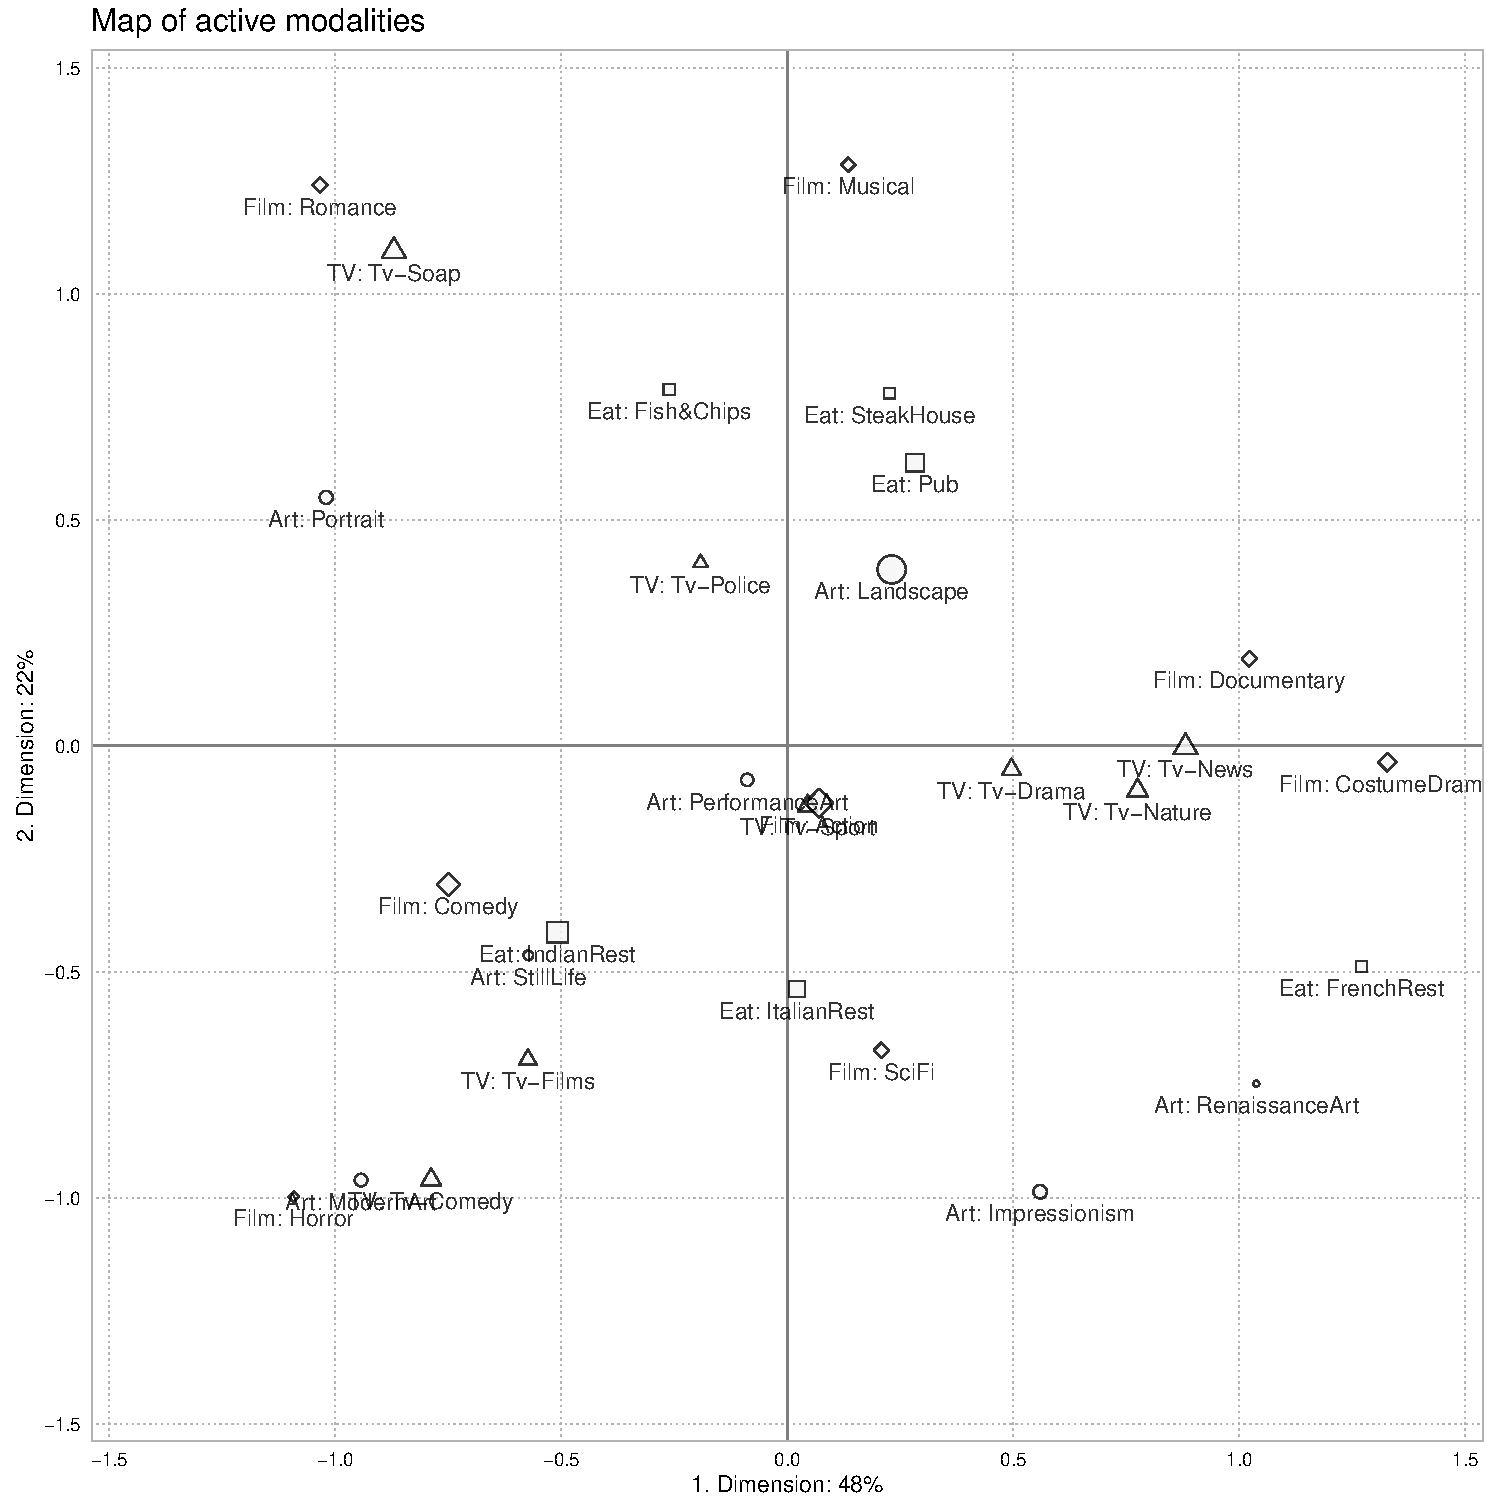
\includegraphics[width=0.75\textwidth,height=\textheight]{ctrl+R_files/figure-pdf/unnamed-chunk-9-1.pdf}

}

\caption{Cloud of active modalities. The first dimension is shown
horizontally, and the second dimension is shown vertically.}

\end{figure}%

\normalsize

\subsubsection{Cloud of contributive
modalities}\label{cloud-of-contributive-modalities}

\scriptsize

\begin{Shaded}
\begin{Highlighting}[]
\FunctionTok{map.ctr}\NormalTok{(}
\NormalTok{  result,}
  \AttributeTok{dim =} \FunctionTok{c}\NormalTok{(}\DecValTok{1}\NormalTok{, }\DecValTok{2}\NormalTok{),}
  \AttributeTok{point.shape =} \StringTok{"variable"}\NormalTok{,}
  \AttributeTok{point.alpha =} \FloatTok{0.8}\NormalTok{,}
  \AttributeTok{point.fill =} \StringTok{"whitesmoke"}\NormalTok{,}
  \AttributeTok{point.color =} \StringTok{"black"}\NormalTok{,}
  \AttributeTok{point.size =} \StringTok{"freq"}\NormalTok{,}
  \AttributeTok{label =} \ConstantTok{TRUE}\NormalTok{,}
  \AttributeTok{label.repel =} \ConstantTok{FALSE}\NormalTok{,}
  \AttributeTok{label.alpha =} \FloatTok{0.8}\NormalTok{,}
  \AttributeTok{label.color =} \StringTok{"black"}\NormalTok{,}
  \AttributeTok{label.size =} \DecValTok{4}\NormalTok{,}
  \AttributeTok{label.fill =} \ConstantTok{NULL}\NormalTok{,}
  \AttributeTok{map.title =} \StringTok{"active"}\NormalTok{,}
  \AttributeTok{labelx =} \StringTok{"default"}\NormalTok{,}
  \AttributeTok{labely =} \StringTok{"default"}\NormalTok{,}
  \AttributeTok{legend =} \ConstantTok{NULL}
\NormalTok{) }\SpecialCharTok{+} \FunctionTok{xlim}\NormalTok{(}\SpecialCharTok{{-}}\FloatTok{1.4}\NormalTok{,}\FloatTok{1.4}\NormalTok{) }\SpecialCharTok{+} \FunctionTok{ylim}\NormalTok{(}\SpecialCharTok{{-}}\FloatTok{1.4}\NormalTok{,}\FloatTok{1.4}\NormalTok{)}
\end{Highlighting}
\end{Shaded}

\begin{figure}[H]

{\centering 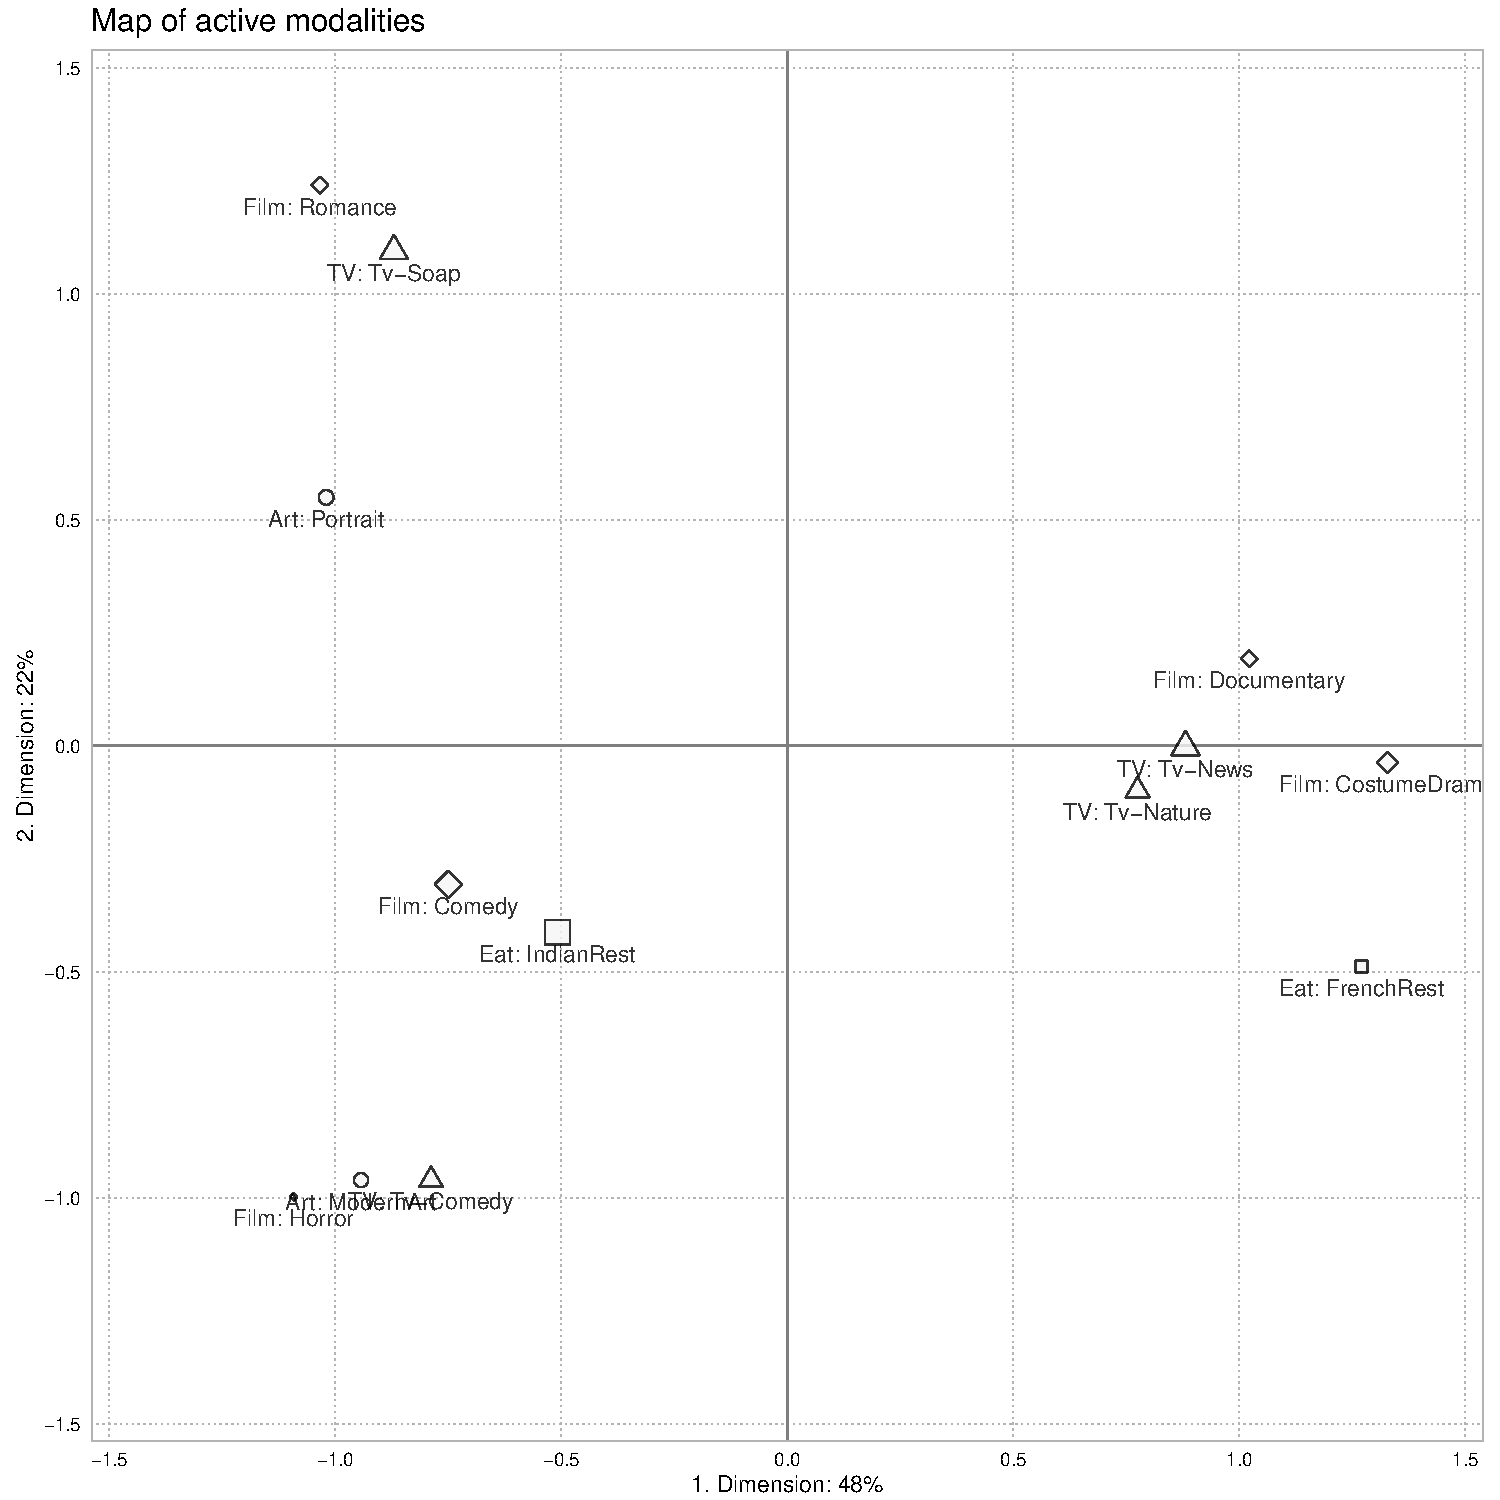
\includegraphics[width=0.75\textwidth,height=\textheight]{ctrl+R_files/figure-pdf/unnamed-chunk-10-1.pdf}

}

\caption{Cloud of contributive modalities. The first dimension is shown
horizontally, and the second dimension is shown vertically.}

\end{figure}%

\normalsize

\subsubsection{Cloud of supplementary
modalities}\label{cloud-of-supplementary-modalities}

\scriptsize

\begin{Shaded}
\begin{Highlighting}[]
\FunctionTok{map.sup}\NormalTok{(}
\NormalTok{  result,}
  \AttributeTok{dim =} \FunctionTok{c}\NormalTok{(}\DecValTok{1}\NormalTok{, }\DecValTok{2}\NormalTok{),}
  \AttributeTok{point.shape =} \StringTok{"variable"}\NormalTok{,}
  \AttributeTok{point.alpha =} \FloatTok{0.8}\NormalTok{,}
  \AttributeTok{point.fill =} \StringTok{"whitesmoke"}\NormalTok{,}
  \AttributeTok{point.color =} \StringTok{"black"}\NormalTok{,}
  \AttributeTok{point.size =} \StringTok{"freq"}\NormalTok{,}
  \AttributeTok{label =} \ConstantTok{TRUE}\NormalTok{,}
  \AttributeTok{label.repel =} \ConstantTok{FALSE}\NormalTok{,}
  \AttributeTok{label.alpha =} \FloatTok{0.8}\NormalTok{,}
  \AttributeTok{label.color =} \StringTok{"black"}\NormalTok{,}
  \AttributeTok{label.size =} \DecValTok{4}\NormalTok{,}
  \AttributeTok{label.fill =} \ConstantTok{NULL}\NormalTok{,}
  \AttributeTok{map.title =} \StringTok{"active"}\NormalTok{,}
  \AttributeTok{labelx =} \StringTok{"default"}\NormalTok{,}
  \AttributeTok{labely =} \StringTok{"default"}\NormalTok{,}
  \AttributeTok{legend =} \ConstantTok{NULL}
\NormalTok{) }\SpecialCharTok{+} \FunctionTok{xlim}\NormalTok{(}\SpecialCharTok{{-}}\FloatTok{1.4}\NormalTok{,}\FloatTok{1.4}\NormalTok{) }\SpecialCharTok{+} \FunctionTok{ylim}\NormalTok{(}\SpecialCharTok{{-}}\FloatTok{1.4}\NormalTok{,}\FloatTok{1.4}\NormalTok{)}
\end{Highlighting}
\end{Shaded}

\begin{figure}[H]

{\centering 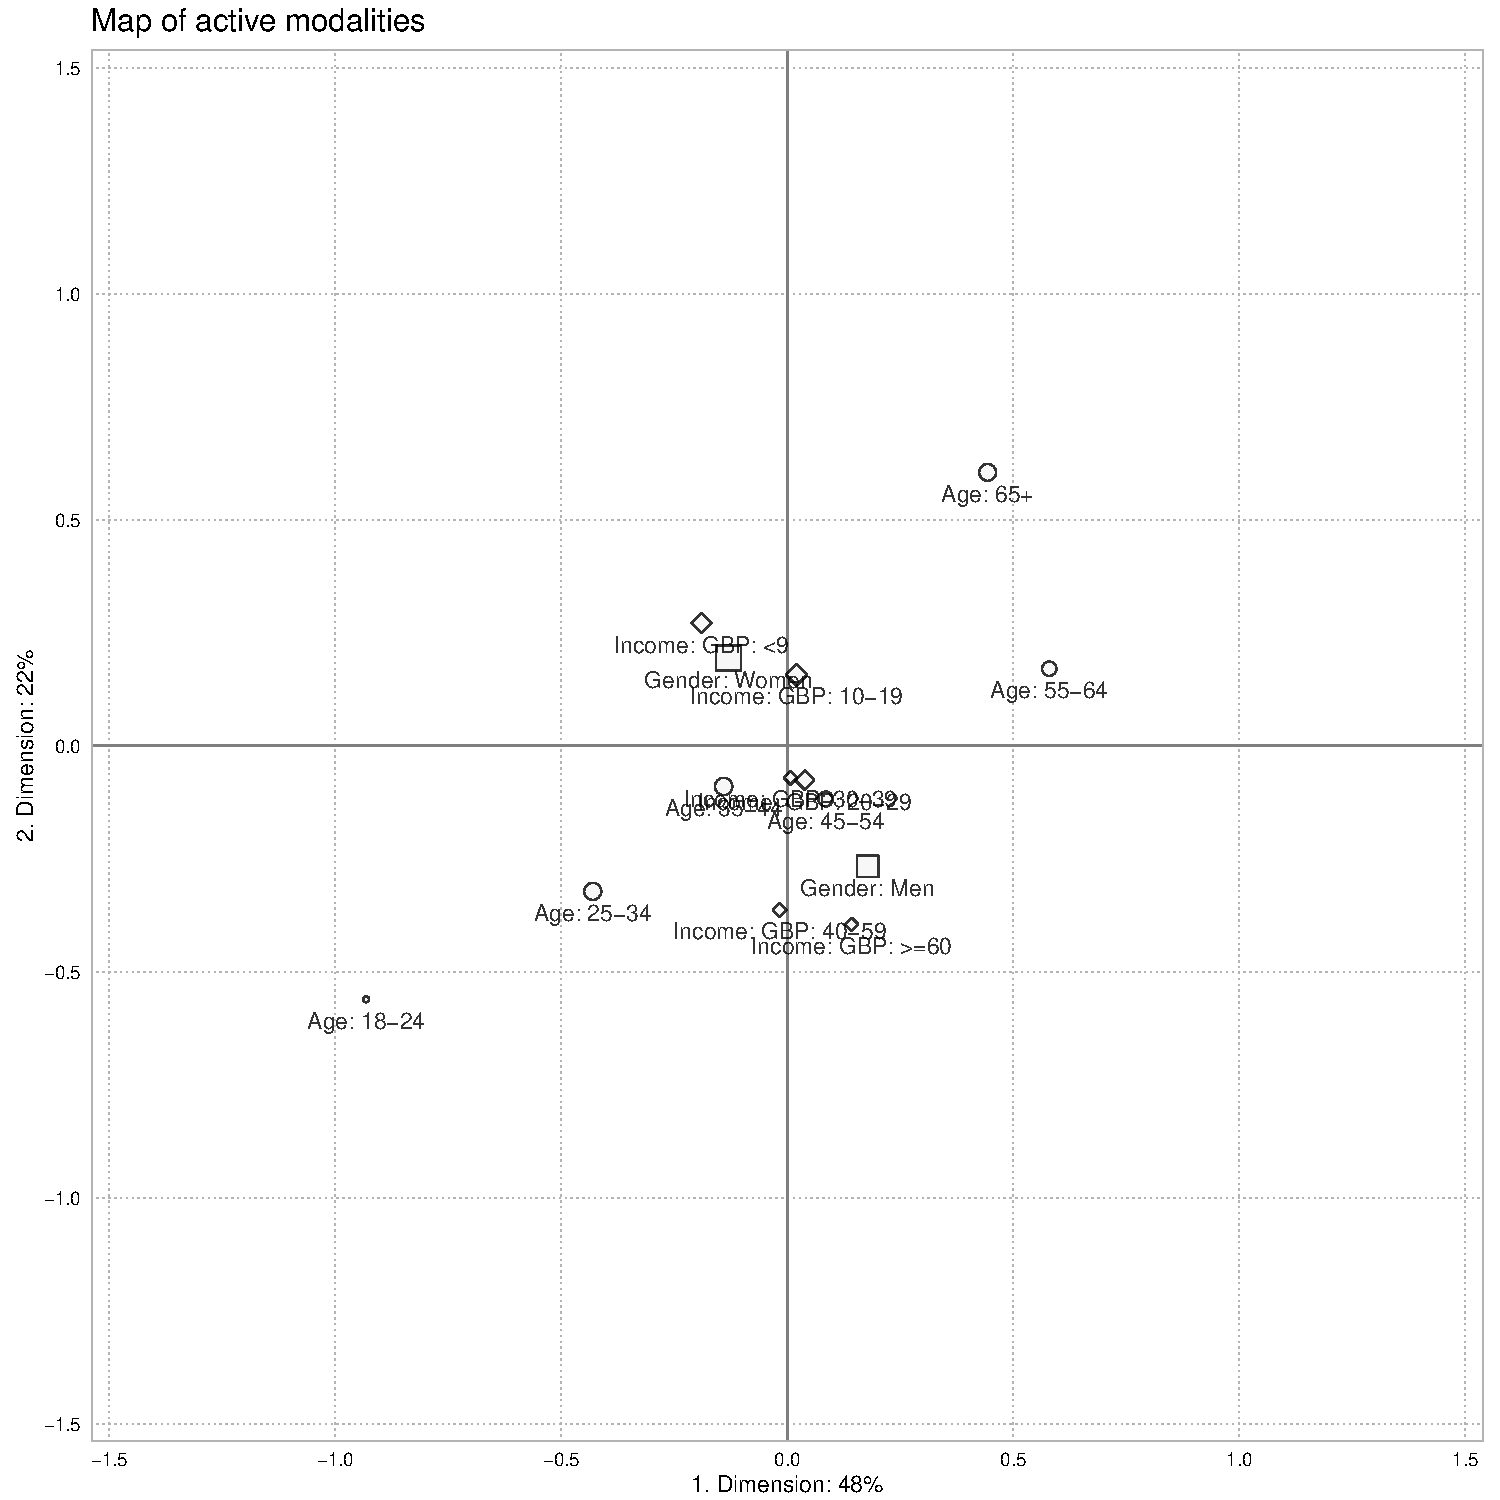
\includegraphics[width=0.75\textwidth,height=\textheight]{ctrl+R_files/figure-pdf/unnamed-chunk-11-1.pdf}

}

\caption{Cloud of supplementary modalities. The first dimension is shown
horizontally, and the second dimension is shown vertically.}

\end{figure}%

\normalsize

\subsubsection{Cloud of individuals}\label{cloud-of-individuals}

\scriptsize

\begin{Shaded}
\begin{Highlighting}[]
\CommentTok{\# map the cloud of individuals}
\NormalTok{map }\OtherTok{\textless{}{-}} \FunctionTok{map.ind}\NormalTok{(result, }\AttributeTok{point.color =} \StringTok{"black"}\NormalTok{, }\AttributeTok{point.size =} \FloatTok{1.5}\NormalTok{, }\AttributeTok{map.title =} \StringTok{""}\NormalTok{)}
\NormalTok{map }\SpecialCharTok{+} \FunctionTok{xlim}\NormalTok{(}\SpecialCharTok{{-}}\FloatTok{1.75}\NormalTok{,}\FloatTok{1.75}\NormalTok{) }\SpecialCharTok{+} \FunctionTok{ylim}\NormalTok{(}\SpecialCharTok{{-}}\FloatTok{1.75}\NormalTok{,}\FloatTok{1.75}\NormalTok{)}
\end{Highlighting}
\end{Shaded}

\begin{figure}[H]

{\centering 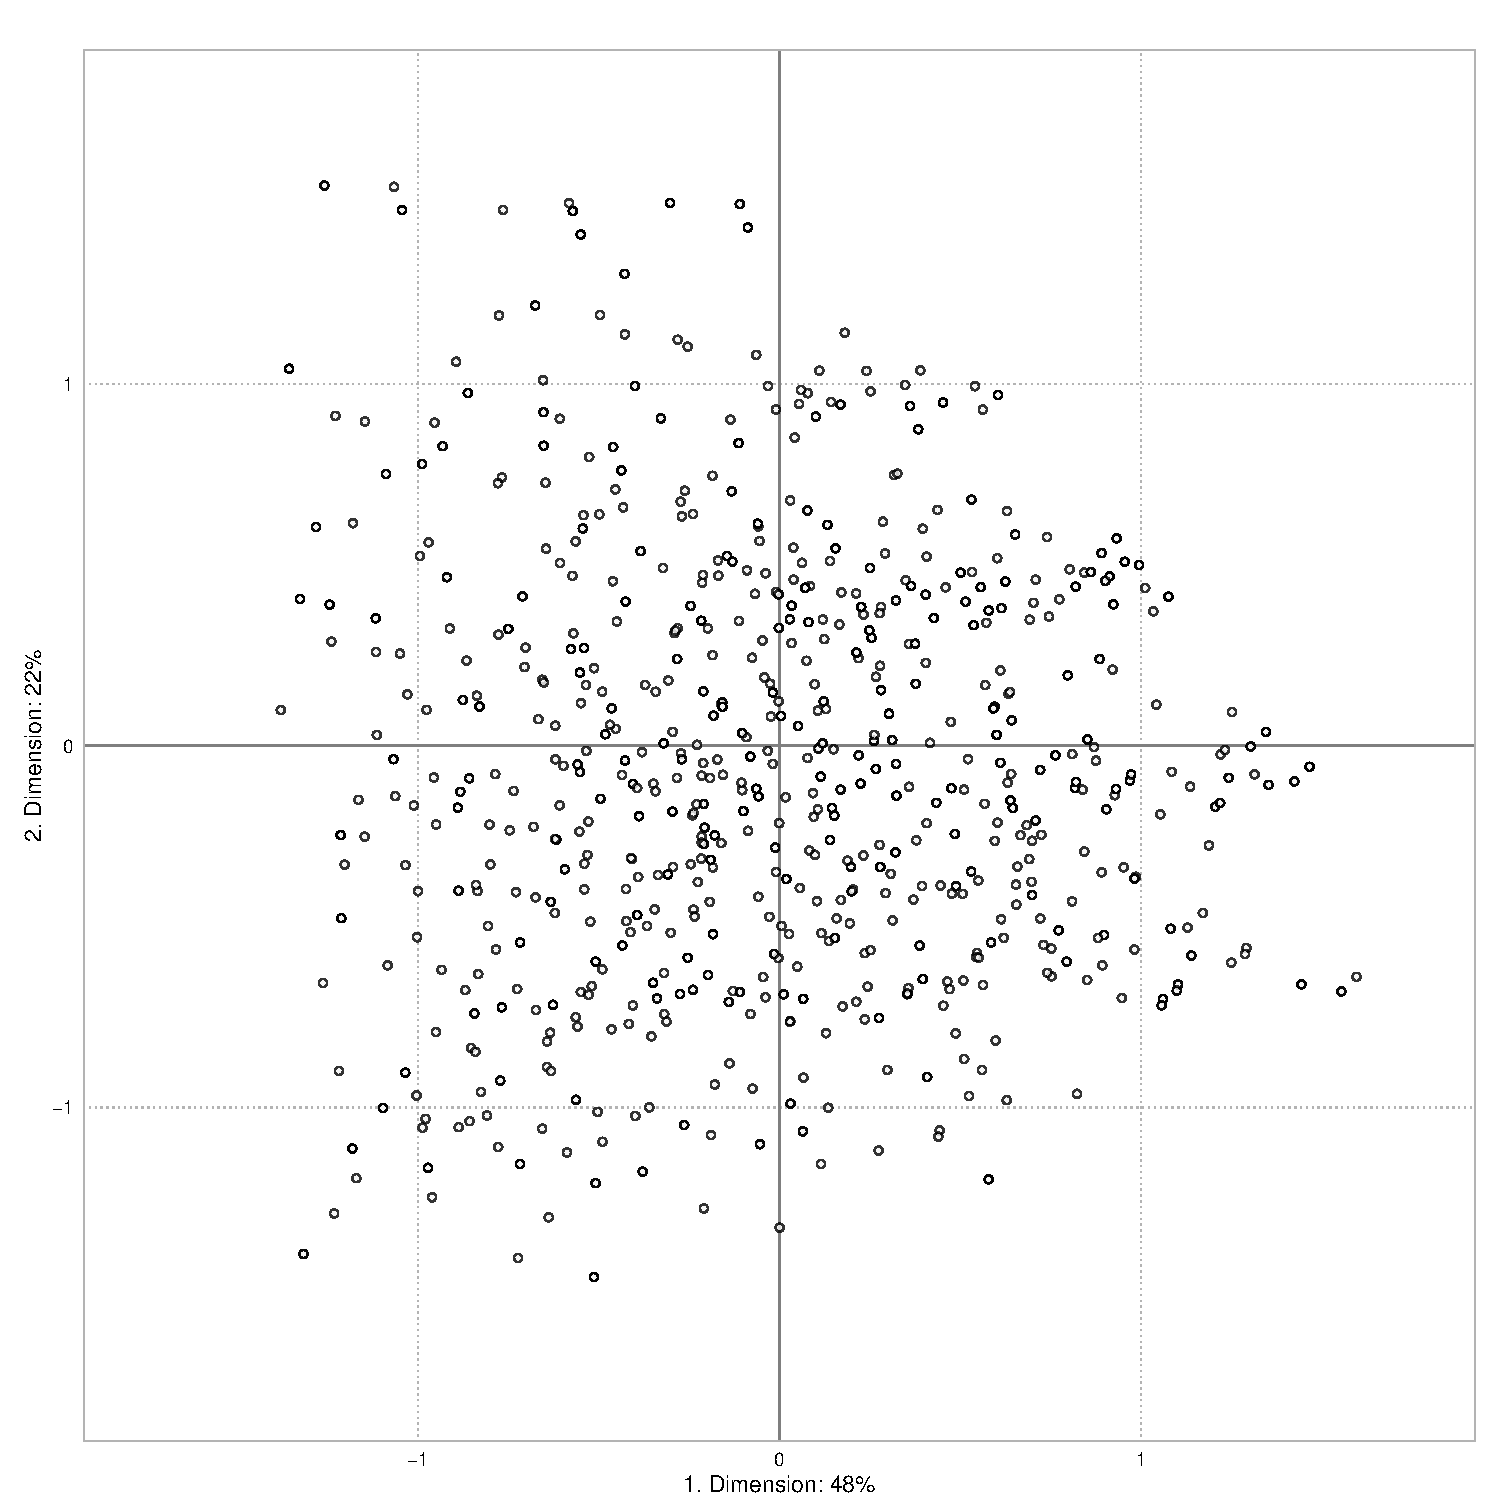
\includegraphics[width=0.75\textwidth,height=\textheight]{ctrl+R_files/figure-pdf/unnamed-chunk-12-1.pdf}

}

\caption{Cloud of individuals. The first dimension is shown
horizontally, and the second dimension is shown vertically.}

\end{figure}%

\normalsize

\subsection{Clustering}\label{clustering}

\scriptsize

\begin{Shaded}
\begin{Highlighting}[]
\FunctionTok{set.seed}\NormalTok{(}\DecValTok{123}\NormalTok{)}

\CommentTok{\# library(factoextra)}

\CommentTok{\# retrieve coordinates of individuals on the three first dimensions}
\NormalTok{coords }\OtherTok{\textless{}{-}}\NormalTok{ result}\SpecialCharTok{$}\NormalTok{coord.ind[, }\DecValTok{1}\SpecialCharTok{:}\DecValTok{3}\NormalTok{]}

\CommentTok{\# optimal number of clusters}
\NormalTok{nbcluters }\OtherTok{\textless{}{-}} \FunctionTok{fviz\_nbclust}\NormalTok{(coords, kmeans, }\AttributeTok{method =} \StringTok{"silhouette"}\NormalTok{) }\CommentTok{\# wss}
\NormalTok{nbcluters}\SpecialCharTok{$}\NormalTok{data}
\end{Highlighting}
\end{Shaded}

\begin{verbatim}
   clusters         y
1         1 0.0000000
2         2 0.2482660
3         3 0.2784929
4         4 0.3188015
5         5 0.2826648
6         6 0.2716818
7         7 0.2616555
8         8 0.2650011
9         9 0.2641515
10       10 0.2528930
\end{verbatim}

\begin{Shaded}
\begin{Highlighting}[]
\NormalTok{nbcluters}
\end{Highlighting}
\end{Shaded}

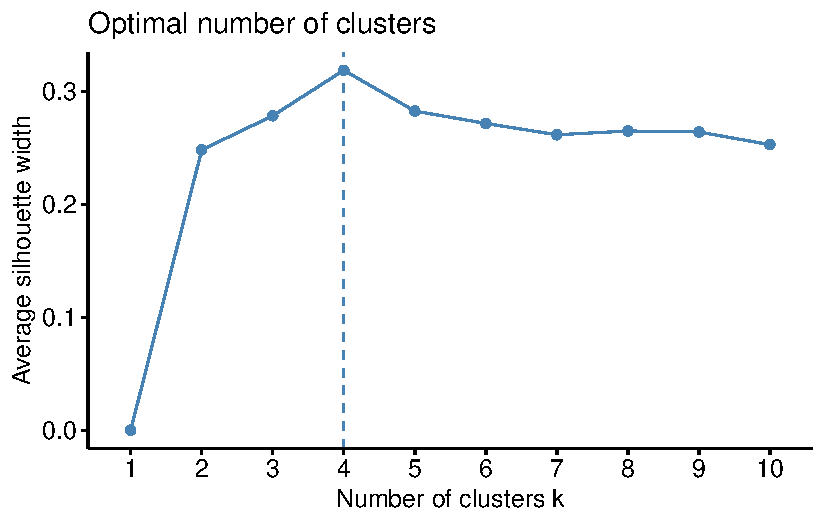
\includegraphics{ctrl+R_files/figure-pdf/unnamed-chunk-13-1.pdf}

\begin{Shaded}
\begin{Highlighting}[]
\CommentTok{\# run k{-}means clustering}
\NormalTok{kmeanclust }\OtherTok{\textless{}{-}} \FunctionTok{kmeans}\NormalTok{(coords, }\DecValTok{4}\NormalTok{, }\AttributeTok{nstart =} \DecValTok{25}\NormalTok{)}
\FunctionTok{table}\NormalTok{(kmeanclust}\SpecialCharTok{$}\NormalTok{cluster)}
\end{Highlighting}
\end{Shaded}

\begin{verbatim}

  1   2   3   4 
294 434 239 248 
\end{verbatim}

\begin{Shaded}
\begin{Highlighting}[]
\NormalTok{taste}\SpecialCharTok{$}\NormalTok{kmeanclust }\OtherTok{\textless{}{-}} \FunctionTok{as.factor}\NormalTok{(kmeanclust}\SpecialCharTok{$}\NormalTok{cluster)}
\FunctionTok{table}\NormalTok{(taste}\SpecialCharTok{$}\NormalTok{kmeanclust)}
\end{Highlighting}
\end{Shaded}

\begin{verbatim}

  1   2   3   4 
294 434 239 248 
\end{verbatim}

\normalsize

\subsubsection{Plot clusters}\label{plot-clusters}

\scriptsize

\begin{Shaded}
\begin{Highlighting}[]
\NormalTok{plot }\OtherTok{\textless{}{-}} \FunctionTok{map.ind}\NormalTok{(result, }\AttributeTok{point.fill =} \FunctionTok{as.factor}\NormalTok{(taste}\SpecialCharTok{$}\NormalTok{kmeanclust), }\AttributeTok{point.size =} \FloatTok{2.5}\NormalTok{)}
\NormalTok{palette }\OtherTok{\textless{}{-}} \FunctionTok{c}\NormalTok{(}\StringTok{"coral2"}\NormalTok{, }\StringTok{"deepskyblue3"}\NormalTok{, }\StringTok{"green"}\NormalTok{, }\StringTok{"grey20"}\NormalTok{)}
\NormalTok{plot }\SpecialCharTok{+} \FunctionTok{scale\_fill\_manual}\NormalTok{(}\AttributeTok{values=}\NormalTok{palette) }\SpecialCharTok{+} \FunctionTok{xlim}\NormalTok{(}\SpecialCharTok{{-}}\FloatTok{1.75}\NormalTok{,}\FloatTok{1.75}\NormalTok{) }\SpecialCharTok{+} \FunctionTok{ylim}\NormalTok{(}\SpecialCharTok{{-}}\FloatTok{1.75}\NormalTok{,}\FloatTok{1.75}\NormalTok{)}
\end{Highlighting}
\end{Shaded}

\begin{figure}[H]

{\centering 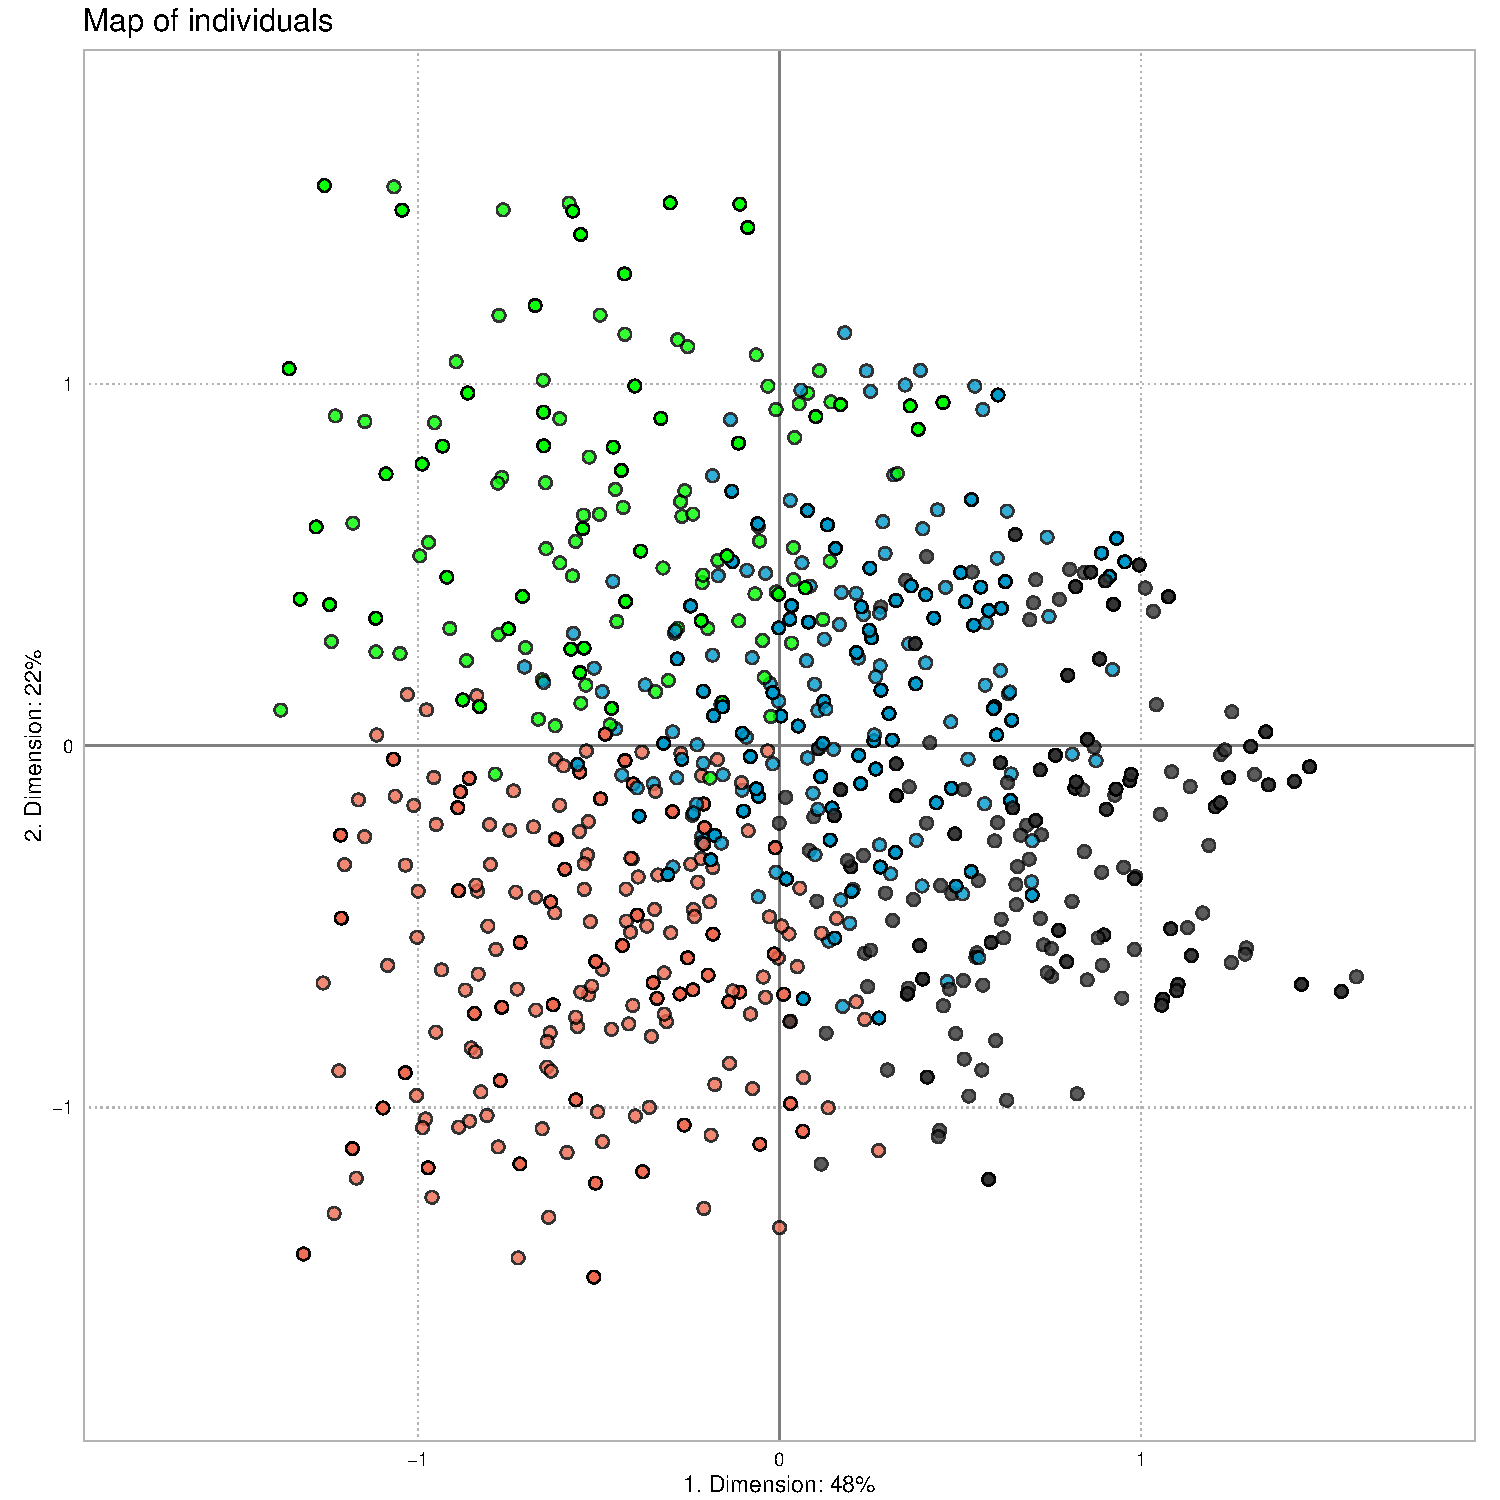
\includegraphics[width=0.75\textwidth,height=\textheight]{ctrl+R_files/figure-pdf/unnamed-chunk-14-1.pdf}

}

\caption{Cluster plot. The first dimension is shown horizontally, and
the second dimension is shown vertically.}

\end{figure}%

\normalsize

\scriptsize

\begin{Shaded}
\begin{Highlighting}[]
\NormalTok{plot }\OtherTok{\textless{}{-}} \FunctionTok{map.ellipse}\NormalTok{(result, map, taste}\SpecialCharTok{$}\NormalTok{kmeanclust, }\AttributeTok{draw.levels =} \DecValTok{1}\SpecialCharTok{:}\FunctionTok{nlevels}\NormalTok{(taste}\SpecialCharTok{$}\NormalTok{kmeanclust), }\AttributeTok{label.size =} \DecValTok{5}\NormalTok{)}
\NormalTok{palette }\OtherTok{\textless{}{-}} \FunctionTok{c}\NormalTok{(}\StringTok{"coral2"}\NormalTok{, }\StringTok{"deepskyblue3"}\NormalTok{, }\StringTok{"green"}\NormalTok{, }\StringTok{"grey20"}\NormalTok{)}
\NormalTok{plot }\SpecialCharTok{+} \FunctionTok{scale\_fill\_manual}\NormalTok{(}\AttributeTok{values=}\NormalTok{palette) }\SpecialCharTok{+} \FunctionTok{xlim}\NormalTok{(}\SpecialCharTok{{-}}\FloatTok{1.75}\NormalTok{,}\FloatTok{1.75}\NormalTok{) }\SpecialCharTok{+} \FunctionTok{ylim}\NormalTok{(}\SpecialCharTok{{-}}\FloatTok{1.75}\NormalTok{,}\FloatTok{1.75}\NormalTok{) }\SpecialCharTok{+} \FunctionTok{labs}\NormalTok{(}\AttributeTok{x =} \StringTok{"Dimension 1 (63.5\%)"}\NormalTok{, }\AttributeTok{y =} \StringTok{"Dimension 2 (16.9\%)"}\NormalTok{)}
\end{Highlighting}
\end{Shaded}

\begin{figure}[H]

{\centering 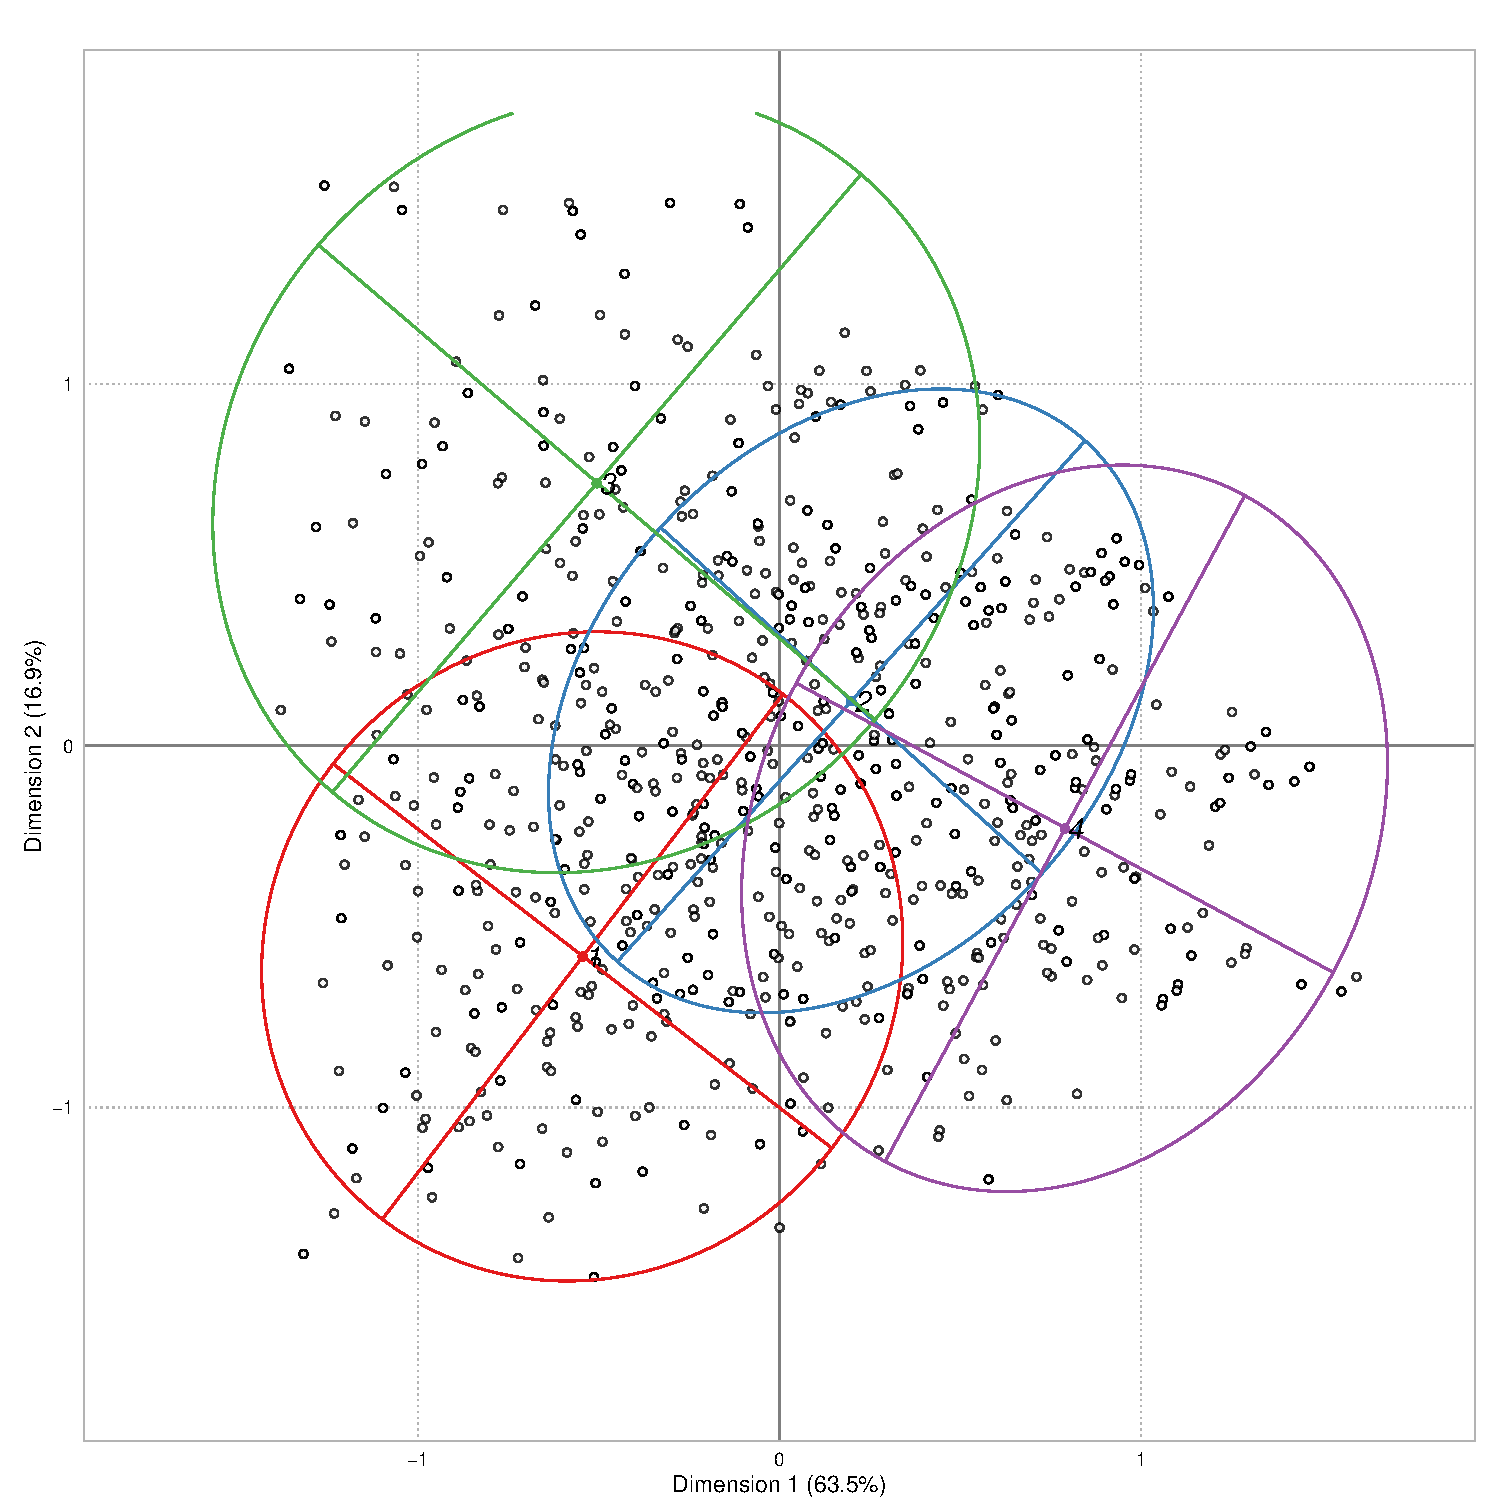
\includegraphics[width=0.75\textwidth,height=\textheight]{ctrl+R_files/figure-pdf/unnamed-chunk-15-1.pdf}

}

\caption{Cluster plot with concentration ellipses. The first dimension
is shown horizontally, and the second dimension is shown vertically.}

\end{figure}%

\normalsize

\subsubsection{Inspect the distribution of the modalities in the
clusters}\label{inspect-the-distribution-of-the-modalities-in-the-clusters}

\scriptsize

\begin{Shaded}
\begin{Highlighting}[]
\CommentTok{\# we look for over / under{-}representations of the modalities. }
\CommentTok{\# for furher information on the method, see FactoMineR documentation. }
\CommentTok{\# see also: Husson, F., Lê, S., \& Pagès, J. (2017). Exploratory multivariate analysis by example using R. Boca Raton: CRC press.}

\CommentTok{\# library(FactoMineR)}
\FunctionTok{names}\NormalTok{(taste)}
\end{Highlighting}
\end{Shaded}

\begin{verbatim}
 [1] "ID"         "Isup"       "TV"         "Film"       "Art"       
 [6] "Eat"        "Gender"     "Age"        "Income"     "kmeanclust"
\end{verbatim}

\begin{Shaded}
\begin{Highlighting}[]
\FunctionTok{catdes}\NormalTok{(taste, }\DecValTok{10}\NormalTok{, }\AttributeTok{proba =} \FloatTok{0.05}\NormalTok{) }\CommentTok{\# clusters}
\end{Highlighting}
\end{Shaded}

\begin{verbatim}

Link between the cluster variable and the categorical variables (chi-square test)
=================================================================================
             p.value df
TV     3.968340e-259 21
Film   2.730812e-230 21
Art     1.399512e-96 18
Eat     5.840889e-85 15
Gender  7.275369e-40  3
Age     3.268215e-33 15
Isup    2.780583e-17  3
Income  7.060819e-05 18

Description of each cluster by the categories
=============================================
$`1`
                    Cla/Mod    Mod/Cla    Global      p.value     v.test
TV=Tv-Comedy      78.947368 40.8163265 12.510288 6.340785e-54  15.461198
Art=ModernArt     70.909091 26.5306122  9.053498 9.607766e-28  10.916549
Film=Comedy       53.191489 42.5170068 19.341564 1.586725e-27  10.870875
Film=Horror       82.258065 17.3469388  5.102881 4.609678e-23   9.889796
Eat=IndianRest    40.298507 55.1020408 33.086420 2.243737e-19   9.000656
TV=Tv-Films       54.700855 21.7687075  9.629630 7.293059e-14   7.482484
Age=18-24         55.913978 17.6870748  7.654321 8.570962e-12   6.828663
Age=25-34         39.919355 33.6734694 20.411523 5.104958e-10   6.215844
Art=StillLife     54.929577 13.2653061  5.843621 1.095436e-08   5.715249
Eat=ItalianRest   34.649123 26.8707483 18.765432 7.481028e-05   3.960445
Income=GBP: 40-59 33.070866 14.2857143 10.452675 1.675771e-02   2.391981
TV=Tv-Drama       17.164179  7.8231293 11.028807 3.988402e-02  -2.054948
Film=Action       19.794344 26.1904762 32.016461 1.318817e-02  -2.478647
Eat=Fish&Chips    11.214953  4.0816327  8.806584 4.933092e-04  -3.484363
Eat=SteakHouse     7.142857  2.3809524  8.065844 6.050295e-06  -4.524624
TV=Tv-Sport        9.558824  4.4217687 11.193416 5.228437e-06  -4.555406
TV=Tv-Soap        11.162791  8.1632653 17.695473 1.790683e-07  -5.219850
Eat=FrenchRest     5.050505  1.7006803  8.148148 1.673494e-07  -5.232371
Film=Romance       4.950495  1.7006803  8.312757 1.010779e-07  -5.324775
Film=Musical       3.448276  1.0204082  7.160494 6.680387e-08  -5.399562
TV=Tv-Nature       7.547170  4.0816327 13.086420 8.113459e-09  -5.766084
TV=Tv-News         9.090909  6.8027211 18.106996 4.612339e-10  -6.231757
Film=Documentary   2.000000  0.6802721  8.230453 1.631033e-10  -6.392586
Age=55-64          7.103825  4.4217687 15.061728 1.158034e-10  -6.444734
Eat=Pub           10.320285  9.8639456 23.127572 4.517586e-11  -6.586025
Film=CostumeDrama  2.142857  1.0204082 11.522634 2.268351e-14  -7.634422
Age=65+            6.611570  5.4421769 19.917695 4.019123e-15  -7.854331
Art=Landscape     11.867089 25.5102041 52.016461 3.779359e-26 -10.577747

$`2`
                     Cla/Mod   Mod/Cla    Global      p.value     v.test
TV=Tv-Sport        86.764706 27.188940 11.193416 4.190921e-39  13.081677
Art=Landscape      51.898734 75.576037 52.016461 1.281665e-35  12.456958
Film=Action        59.897172 53.686636 32.016461 6.806046e-33  11.946080
Gender=Men         52.826511 62.442396 42.222222 2.078570e-26  10.633632
Eat=SteakHouse     63.265306 14.285714  8.065844 8.492344e-09   5.758383
Eat=Pub            50.177936 32.488479 23.127572 1.372024e-08   5.676844
Film=Documentary   61.000000 14.055300  8.230453 8.986277e-08   5.346114
TV=Tv-Nature       54.716981 20.046083 13.086420 1.642287e-07   5.235848
TV=Tv-News         45.909091 23.271889 18.106996 5.934130e-04   3.434607
Film=SciFi         51.485149 11.981567  8.312757 7.501552e-04   3.370560
TV=Tv-Police       52.439024  9.907834  6.748971 1.435781e-03   3.187360
Age=65+            44.214876 24.654378 19.917695 2.332961e-03   3.044205
Age=55-64          43.169399 18.202765 15.061728 2.414632e-02   2.254793
Eat=Fish&Chips     44.859813 11.059908  8.806584 4.199429e-02   2.033577
Eat=IndianRest     31.094527 28.801843 33.086420 1.768081e-02  -2.372236
Art=Portrait       25.641026  6.912442  9.629630 1.523221e-02  -2.426811
Art=StillLife      21.126761  3.456221  5.843621 6.712151e-03  -2.710798
Age=18-24          21.505376  4.608295  7.654321 2.247176e-03  -3.055457
Age=25-34          25.806452 14.746544 20.411523 2.092579e-04  -3.707570
Art=RenaissanceArt 12.727273  1.612903  4.526749 1.119971e-04  -3.863013
TV=Tv-Drama        17.910448  5.529954 11.028807 1.999985e-06  -4.753426
Film=Horror         8.064516  1.152074  5.102881 3.359682e-07  -5.102064
Eat=ItalianRest    21.491228 11.290323 18.765432 3.167599e-07  -5.113192
Film=Comedy        19.574468 10.599078 19.341564 2.737618e-09  -5.946605
Eat=FrenchRest      9.090909  2.073733  8.148148 3.219390e-10  -6.287828
Art=Impressionism  11.200000  3.225806 10.288066 8.080573e-11  -6.499093
Art=ModernArt       6.363636  1.612903  9.053498 6.720005e-14  -7.493228
TV=Tv-Comedy        9.868421  3.456221 12.510288 1.291362e-14  -7.706677
Film=Romance        0.000000  0.000000  8.312757 3.431967e-21  -9.448660
Film=CostumeDrama   2.857143  0.921659 11.522634 3.292343e-23  -9.923433
Gender=Women       23.219373 37.557604 57.777778 2.078570e-26 -10.633632
TV=Tv-Soap          2.790698  1.382488 17.695473 5.627668e-37 -12.703870

$`3`
                      Cla/Mod    Mod/Cla    Global       p.value     v.test
TV=Tv-Soap         82.7906977 74.4769874 17.695473 1.407754e-120  23.349092
Film=Romance       89.1089109 37.6569038  8.312757  1.096386e-57  16.009528
Gender=Women       30.9116809 90.7949791 57.777778  2.663256e-35  12.398481
Art=Portrait       44.4444444 21.7573222  9.629630  1.116718e-10   6.450242
Film=Musical       45.9770115 16.7364017  7.160494  7.482765e-09   5.779714
Eat=Fish&Chips     35.5140187 15.8995816  8.806584  5.716134e-05   4.024233
Income=GBP: <9     27.7056277 26.7782427 19.012346  9.628903e-04   3.301151
Eat=Pub            24.9110320 29.2887029 23.127572  1.354351e-02   2.469148
Film=Horror         9.6774194  2.5104603  5.102881  3.371321e-02  -2.123485
Income=GBP: >=60   11.4754098  5.8577406 10.041152  1.249750e-02  -2.497776
Income=GBP: 40-59  10.2362205  5.4393305 10.452675  2.913037e-03  -2.976769
Art=RenaissanceArt  3.6363636  0.8368201  4.526749  5.580991e-04  -3.451200
Film=CostumeDrama   8.5714286  5.0209205 11.522634  1.670166e-04  -3.764299
Film=Documentary    6.0000000  2.5104603  8.230453  7.575505e-05  -3.957447
Eat=FrenchRest      4.0404040  1.6736402  8.148148  3.645881e-06  -4.630611
Art=Impressionism   5.6000000  2.9288703 10.288066  3.512551e-06  -4.638319
TV=Tv-Films         5.1282051  2.5104603  9.629630  3.315916e-06  -4.650214
Film=SciFi          3.9603960  1.6736402  8.312757  2.447674e-06  -4.712441
TV=Tv-Comedy        4.6052632  2.9288703 12.510288  1.864657e-08  -5.624111
TV=Tv-Nature        4.4025157  2.9288703 13.086420  4.482853e-09  -5.865313
Film=Action         8.7403599 14.2259414 32.016461  4.266101e-12  -6.928073
TV=Tv-Sport         0.7352941  0.4184100 11.193416  6.226454e-13  -7.195429
TV=Tv-News          2.2727273  2.0920502 18.106996  5.972230e-17  -8.365773
Gender=Men          4.2884990  9.2050209 42.222222  2.663256e-35 -12.398481

$`4`
                     Cla/Mod    Mod/Cla    Global      p.value    v.test
Film=CostumeDrama  86.428571 48.7903226 11.522634 6.528159e-75 18.312913
Eat=FrenchRest     81.818182 32.6612903  8.148148 1.123318e-43 13.858933
Art=Impressionism  55.200000 27.8225806 10.288066 5.894699e-20  9.146245
TV=Tv-News         42.727273 37.9032258 18.106996 2.656048e-17  8.460776
TV=Tv-Drama        49.253731 26.6129032 11.028807 1.512855e-15  7.975891
Art=RenaissanceArt 67.272727 14.9193548  4.526749 1.485181e-14  7.688803
Age=55-64          34.426230 25.4032258 15.061728 1.353239e-06  4.831771
TV=Tv-Nature       33.333333 21.3709677 13.086420 3.935456e-05  4.111237
Eat=ItalianRest    28.070175 25.8064516 18.765432 2.021407e-03  3.087069
Film=Documentary   31.000000 12.5000000  8.230453 8.941723e-03  2.614274
Age=65+            26.446281 25.8064516 19.917695 1.104259e-02  2.541348
Gender=Women       22.792023 64.5161290 57.777778 1.572040e-02  2.415343
Gender=Men         17.153996 35.4838710 42.222222 1.572040e-02 -2.415343
Art=StillLife       8.450704  2.4193548  5.843621 5.956037e-03 -2.750192
Eat=Pub            14.590747 16.5322581 23.127572 4.786440e-03 -2.821066
TV=Tv-Police        8.536585  2.8225806  6.748971 3.131929e-03 -2.954484
Eat=SteakHouse      8.163265  3.2258065  8.065844 7.298010e-04 -3.378132
Eat=Fish&Chips      8.411215  3.6290323  8.806584 5.273481e-04 -3.466466
Art=ModernArt       8.181818  3.6290323  9.053498 3.223754e-04 -3.596623
Age=25-34          12.096774 12.0967742 20.411523 1.521173e-04 -3.787587
Art=Landscape      15.981013 40.7258065 52.016461 6.783415e-05 -3.983757
Film=Romance        5.940594  2.4193548  8.312757 3.077751e-05 -4.167636
Income=GBP: <9     10.822511 10.0806452 19.012346 2.409758e-05 -4.223090
TV=Tv-Films         5.982906  2.8225806  9.629630 6.560895e-06 -4.507458
TV=Tv-Comedy        6.578947  4.0322581 12.510288 6.679024e-07 -4.970472
Film=Horror         0.000000  0.0000000  5.102881 4.703968e-07 -5.038010
Film=Action        11.568123 18.1451613 32.016461 5.525530e-08 -5.433513
Age=18-24           1.075269  0.4032258  7.654321 6.539870e-09 -5.802333
Eat=IndianRest     11.194030 18.1451613 33.086420 6.249153e-09 -5.809950
Art=Portrait        2.564103  1.2096774  9.629630 4.043408e-09 -5.882408
Film=Comedy         7.234043  6.8548387 19.341564 1.357776e-09 -6.060407
TV=Tv-Sport         2.941176  1.6129032 11.193416 5.024974e-10 -6.218323
TV=Tv-Soap          3.255814  2.8225806 17.695473 3.089766e-15 -7.887226
\end{verbatim}

\begin{Shaded}
\begin{Highlighting}[]
\CommentTok{\# alternatively, univariate analysis for gender}
\FunctionTok{catdes}\NormalTok{(taste, }\DecValTok{7}\NormalTok{, }\AttributeTok{proba =} \FloatTok{0.05}\NormalTok{) }\CommentTok{\# gender}
\end{Highlighting}
\end{Shaded}

\begin{verbatim}

Link between the cluster variable and the categorical variables (chi-square test)
=================================================================================
                p.value df
TV         2.083150e-63  7
kmeanclust 7.275369e-40  3
Film       2.271438e-37  7
Isup       5.887764e-08  1
Income     4.651985e-05  6
Art        7.814206e-03  6

Description of each cluster by the categories
=============================================
$Men
                    Cla/Mod    Mod/Cla    Global      p.value     v.test
TV=Tv-Sport       90.441176 23.9766082 11.193416 1.033381e-35  12.474123
kmeanclust=2      62.442396 52.8265107 35.720165 2.078570e-26  10.633632
Film=Action       57.583548 43.6647173 32.016461 1.279207e-13   7.408308
Film=SciFi        69.306931 13.6452242  8.312757 1.140295e-08   5.708420
Film=Documentary  60.000000 11.6959064  8.230453 2.054019e-04   3.712278
TV=Tv-Nature      55.345912 17.1539961 13.086420 3.720101e-04   3.559183
Income=GBP: >=60  57.377049 13.6452242 10.041152 4.096157e-04   3.533810
TV=Tv-Comedy      53.289474 15.7894737 12.510288 3.433086e-03   2.926038
TV=Tv-News        50.909091 21.8323587 18.106996 4.207841e-03   2.862145
Art=Landscape     45.886076 56.5302144 52.016461 7.152752e-03   2.689648
Income=GBP: 40-59 51.181102 12.6705653 10.452675 3.229190e-02   2.140779
Income=GBP: <9    35.930736 16.1793372 19.012346 3.108058e-02  -2.156039
Film=Comedy       35.744681 16.3742690 19.341564 2.482260e-02  -2.244152
Income=GBP: 10-19 35.856574 17.5438596 20.658436 2.156345e-02  -2.297971
kmeanclust=4      35.483871 17.1539961 20.411523 1.572040e-02  -2.415343
TV=Tv-Police      25.609756  4.0935673  6.748971 1.333886e-03  -3.208588
Film=Musical      25.287356  4.2884990  7.160494 7.230212e-04  -3.380697
Art=Portrait      27.350427  6.2378168  9.629630 5.037304e-04  -3.478765
TV=Tv-Drama       17.164179  4.4834308 11.028807 7.906399e-11  -6.502371
Film=CostumeDrama 17.142857  4.6783626 11.522634 2.543093e-11  -6.670860
Film=Romance       4.950495  0.9746589  8.312757 1.253851e-18  -8.809786
kmeanclust=3       9.205021  4.2884990 19.670782 2.663256e-35 -12.398481
TV=Tv-Soap         6.511628  2.7290448 17.695473 2.045338e-37 -12.782814

$Women
                    Cla/Mod   Mod/Cla    Global      p.value     v.test
TV=Tv-Soap        93.488372 28.632479 17.695473 2.045338e-37  12.782814
kmeanclust=3      90.794979 30.911681 19.670782 2.663256e-35  12.398481
Film=Romance      95.049505 13.675214  8.312757 1.253851e-18   8.809786
Film=CostumeDrama 82.857143 16.524217 11.522634 2.543093e-11   6.670860
TV=Tv-Drama       82.835821 15.811966 11.028807 7.906399e-11   6.502371
Art=Portrait      72.649573 12.108262  9.629630 5.037304e-04   3.478765
Film=Musical      74.712644  9.259259  7.160494 7.230212e-04   3.380697
TV=Tv-Police      74.390244  8.689459  6.748971 1.333886e-03   3.208588
kmeanclust=4      64.516129 22.792023 20.411523 1.572040e-02   2.415343
Income=GBP: 10-19 64.143426 22.934473 20.658436 2.156345e-02   2.297971
Film=Comedy       64.255319 21.509972 19.341564 2.482260e-02   2.244152
Income=GBP: <9    64.069264 21.082621 19.012346 3.108058e-02   2.156039
Income=GBP: 40-59 48.818898  8.831909 10.452675 3.229190e-02  -2.140779
Art=Landscape     54.113924 48.717949 52.016461 7.152752e-03  -2.689648
TV=Tv-News        49.090909 15.384615 18.106996 4.207841e-03  -2.862145
TV=Tv-Comedy      46.710526 10.113960 12.510288 3.433086e-03  -2.926038
Income=GBP: >=60  42.622951  7.407407 10.041152 4.096157e-04  -3.533810
TV=Tv-Nature      44.654088 10.113960 13.086420 3.720101e-04  -3.559183
Film=Documentary  40.000000  5.698006  8.230453 2.054019e-04  -3.712278
Film=SciFi        30.693069  4.415954  8.312757 1.140295e-08  -5.708420
Film=Action       42.416452 23.504274 32.016461 1.279207e-13  -7.408308
kmeanclust=2      37.557604 23.219373 35.720165 2.078570e-26 -10.633632
TV=Tv-Sport        9.558824  1.851852 11.193416 1.033381e-35 -12.474123
\end{verbatim}

\normalsize

In here, we are interested in the distribution of each modality in each
cluster (or any other variable, e.g., gender) according to the
proportion of individuals characterized by the modality who also belong
to the class and the proportion of the modality in the general
population (Husson et al., 2017). For each modality, a p-value and a
test-value (v-test) indicate the probability that the class distribution
is not due to chance. It is thus the equivalent of a test for comparing
averages when the variable is quantitative, and a test for comparing
proportions when the variable is categorical. The p-value threshold is
set at 0.05 and corresponds to a test value of + or - 2. The latter has
a sign, a positive sign meaning that the modality is over-represented in
the class, a negative sign that it is under-represented. The v-test thus
makes it possible to sort the modalities in order of importance for
their contribution to the class.

\subsection{References}\label{references}

Hjellbrekke, J. (2018). \emph{Multiple correspondence analysis for the
social sciences}. Routledge.

Husson, F., Le, S. and Pages, J. (2017). \emph{Exploratory Multivariate
Analysis by Example Using R.} Boca Raton: CRC Press Book.

Larsen, A. G., et al.~(2021) Package `soc.ca': Specific Correspondence
Analysis for the Social Sciences. Available at:
\url{https://cran.r-project.org/web/packages/soc.ca/index.html}

Le, S., Josse, J. \& Husson, F. (2008). FactoMineR: An R Package for
Multivariate Analysis. Journal of Statistical Software. 25(1). pp.~1-18.
\url{https://www.jstatsoft.org/v25/i01/}. A website:
\url{http://factominer.free.fr/}

Le Roux, B., \& Rouanet, H. (2010). Multiple correspondence analysis.
Thousand Oaks: Sage.




\end{document}
